%%
%% neuralfields.tex
%% 
%% Made by jjfigueredou
%% Login   <jjfigueredou@fctp-jjfu>
%% 
%% Started on  Sun Oct  5 12:26:22 2008 jjfigueredou
%% Last update Sun Oct  5 12:26:22 2008 jjfigueredou
%%
\documentclass[conference]{IEEEtran}
%\documentclass[preprint]{sigplanconf}
\usepackage{stmaryrd}
\usepackage{amsfonts}

\usepackage[latin1]{inputenc}
\usepackage[numbers]{natbib}
\usepackage[english]{babel}
\usepackage{graphicx}
\usepackage{algorithm}
\usepackage{algorithmic}
\usepackage{amsmath}

\hyphenation{op-tical net-works semi-conduc-tor IEEEtran}

\IEEEoverridecommandlockouts    % to create the author's affliation portion
                % using \thanks

\textwidth 178mm    % <------ These are the adjustments we made 10/18/2005
\textheight 239mm   % You may or may not need to adjust these numbes again
\oddsidemargin -7mm
\evensidemargin -7mm
\topmargin -6mm
\columnsep 5mm


\begin{document}

\title{\ \\ \LARGE\bf Neural Fields Applied to the Stability Problem
  of a Simple Biped Walking Model \thanks{Juan Figueredo and Jonatan
    G�mez are with the Department of Systems and Industrial
    Engineering, The National University of Colombia, Bogot�, Colombia
    (email: \{jjfigueredou,jgomezpe\}@unal.edu.co).}}

\author{Juan Figueredo and Jonatan G�mez}

\maketitle

\begin{abstract}
  We aim here to propose a control planning system or architecture
  based on neural fields which is suitable to control a relatively
  complex system. We test it over the stability problem on a typical
  inverted-pendulum and compare it against a more traditional
  recurrent neural network controller. First, we present the neural
  fields model, some variations of it which will be useful for its
  evolution and some of the properties that arise from it. Next, we
  study its applications to control and compare it with the recurrent
  neural network control scheme, which is also evolved. Finally we
  test it with the inverted-pendulum problem.
\end{abstract}

\section{Introduction}
Artificial life aims to find those emergent phenomena that give
complex attributes to the existent living beings. In this work,
efforts are directed towards the study of emergence of motion control
capabilities and dynamical planning behaviors of biped walking
agents. Following the artificial life approach
\cite{Nolfi04Evolutionary}, those capabilities are expected to emerge
from a very simple or non-functional initialization, in this case
using a neural control architecture.

In biped robotics, the methods based on computational intelligence for
planning and control, have shown to be able to achieve static
stability \cite{Kun97Adaptive}, dynamical stability
\cite{Nakanishi2004b,Komatsu05Dynamic}, achieve simple control
structures \cite{Huelse04Structure}, and tolerate perturbations
\cite{Juang02Intelligent}. Nonetheless, those properties have not been
extended to an integrated architecture of planning and control capable
of following goals.

Here, there are compared two control schemes based on neural networks
in order to observe their advantages and disadvantages as planning and
control architectures and their suitability as controllers given their
structure. The first one, uses a simple model of recurrent connections
between neurons without additional restrictions, i.e. a recurrent
neural network. The second one, based on neural fields, has a deeper
biological basis, applying more restrictions and extending the
discrete model to a continuous one, following the method of planning
and control by means of neural fields \cite{Bergener99Complex}. The
control problem set for testing the architectures is the stability
problem on a inverted pendulum, so that their ability to perform
dynamic control on an unstable plant can be evaluated. To the authors'
knowledge this is the first time neural fields have been evaluated for
solving a control problem for an unstable plant.

First, some preliminaries on computational intelligence are presented,
mainly in the areas of evolutionary computation, and in the area of
neural controllers, which is the main focus of the article. In the
remaining sections the control problem used as test bed is presented,
an application of traditional evolutionary computation methods is
shown, a co-evolution scheme is applied, other incremental evolution
methods are used to obtain greater complexity, and finally, a
discussion is made.


\section{Preliminaries on Computational Intelligence}
\subsection*{Evolutionary algorithms}
Evolutionary algorithms are a set of population-based heuristic search
and optimization techniques. They maintain a population, and apply a
set of operators or transformations over its members. Those operators
are typically inspired on biological evolution and usually include
selection, reproduction and mutation, among others. The operators are
dependent of the evaluation of a performance function called fitness
function. Generally, fitness function evaluation may include, from a
simple numerical evaluation, to a complex simulation, in order to get
the performance criterion which its optimization is pursued.

The pseudo-code of a general evolutionary algorithm is as follows:

\algsetup{indent=2em}
\begin{algorithm}[h!]
  \caption{$Evolutionary Algorithm$}\label{alg:factorial}
  \begin{algorithmic}[1]
    \STATE $P \leftarrow$ Generate initial population of size $N$
    \STATE Evaluate fitness for each individual in $P$ \REPEAT \STATE
    $P' \leftarrow$ Apply operators to $P$ \STATE Evaluate fitness for
    each individual in $P'$ \STATE $P \leftarrow$ Select $N$
    individuals in $P'$ according to a selection scheme
    \UNTIL{Termination condition is met}
  \end{algorithmic}
\end{algorithm}

The most predominant form of an evolutionary algorithm is embodied by
genetic algorithms. They most frequent genotypical representation is a
bit sequence, although other representations can be used. Usually they
are implemented with a generational replacement of population, but in
some situations it is useful to conserve a small set of the better
individuals across generations in a steady-steady replacement.

\subsection*{Neural networks}
Artificial neural networks are a connectionist computing scheme
inspired by brain neural layout at cellular level. It is based on
simple computing structures called neurons which have several inputs
and a single output.

The particular topologies of interest here are recurrent neural
networks and neural fields.

For recurrent neural networks the model, as is presented in
\cite{Haykin98Neural} is:

\begin{align}
  \begin{split}
    x_{rnn}(n+1)&=\Psi (W_ax_{rnn}(n)+W_bu_{rnn}(n)) \\
    y_{rnn}(n)&=Cx_{rnn}(n)
  \end{split}
\end{align}

Here, $x_{rnn}$ is the 1-by-q system state vector at $n$, $\Psi$ is a
diagonal function with domain and co-domain $R^q$ corresponding to
activation function, $u_{rnn}$ is the 1-by-m input vector at $n$, the
.q-by-q matrix $W_a$ represents the connection weights between
neurons, and the q-by-m+1 matrix represents the connection weights
between input nodes and neurons, including a bias term. Also,
$y_{rnn}$ is the neural output vector of the neural net, and $C$ is a
p-by-q matrix of linear combination from the neurons to the outputs.

Recurrent neural networks present a dynamic behavior because of its
memory, that is, each state depends of the previous state in such a
way that a difference equation arises. Here, there is not a notion of
locality and the interactions between neurons and inputs is given by
parameter matrices.

Neural fields, on the other, hand are tissue level models which
describe the evolution of distributed variables (e.g. the activation
potential). Their mathematical formulation for the one-dimensional
case is:

\begin{equation}
  \label{eq:neuralfield}
  \frac{1}{\alpha}
  \dot{u}(\psi)=-u(\psi)-h+s(\psi)+\int_{-\infty}^{\infty}{w(\psi,\psi')\sigma(u(\psi'))d\psi'}
\end{equation}

The main difference between recurrent neural networks and neural
fields is that, in the first, the relation among the neurons is
arbitrary and discrete, but in the second is continuous and is meant
to be related to locality. Besides, the first right hand element
assures and stable homogeneous behavior in linear form.

\section{Neural Fields for Control and Planning}
For the purpose of control and planning we need some particular
requirements on the neural fields.

The first one is to have a preprocessing over the input obtained from
the sensors, so that there is a closed loop where the representation
of inputs has an appropriate form. This mechanism alone (a particular
form for the inputs) has shown to be enough for the robot ARNOLD to
navigate in the plane with obstacles \cite{Bergener99Complex}.

The second one is to be able to modify the connection kernel so that
it can be suitable to our control problem. In order to do that, we
will consider that the connection kernel $w(y)$ is a symmetric
function (i.e. $w(y)=w(-y)$), that also is a 2-power Lebesgue
integrable function so that it also belong to $L^2$. It can be shown
that, whit that definition, a sum of an arbitrary number of kernel
functions will also be a kernel function. This way, we have a
inner-product defined by the Lebesgue measure:

\begin{equation}
  \label{eq:eq-l2}
  \langle f,g \rangle_{L^2} = \int_{R}{f\cdot g d\mu}
\end{equation}

The defined space, whit its measure, conforms a Hilbert space, and
therefore is complete and metrizable. It also gives a notion of sum,
and scalar product:
\begin{eqnarray}
  \label{eq:eq-leb-opers}
  (f+g)(x)=&f(x)+g(x) \\
  (\lambda f)(x)=&\lambda f(x)
\end{eqnarray}
Those properties will be used shortly when arises the problem kernel
evolution.

The third one consists of its suitability to simulation. This is not
an inherent restriction for it to be physically (or biologically)
plausible, but to be implementable on a computer. We will take a
discrete form of the equation \ref{eq:nf-simp}:


\begin{equation}
  \label{eq:nf-disc}
  \tau \dot{u}_i=-u_i+\sum_{x_j \in B_p(x_i)} {w\left(x_i,x_j\right)
    f\left( u_j \right)}+S(x_i,t)
\end{equation}

Where we replace the integral for a sum over the point included inside
a finite neighborhood (ball) around $x_i$ with radius $p$. The time is
considered continuous, and the computation of the dynamical system
behavior is evaluated with a Runge-Kutta method. We denote
$u_i=u(x_i,t)$. It should be noted that the previous equation can be
applied to the $n$-dimensional case without modification.

\section{Control Architecture}
The control architecture built based on the neural fields has three
basic elements.

The first one, is a sensor, which reads the states from the plant and
also their derivatives (computed from the dynamical equation of the
plant). In particular, the sensor used for the neural field controller
is based on the angular acceleration of the pendulum pole, loosely
resembling the vestibular system on the inner ear.

The second one is the input layer, which consists of a simple neural
field without natural dynamics, where the spatial codification of the
sensed values is made. For the problem at hand, we use a finite
one-dimensional neural field, where a sensed input with value zero
maps to the center point of the field.

The third one is the processing layer, which has a more typical neural
field which has inner dynamics given by the eq. \ref{eq:nf-disc},
where the fields taken into the sum are the input neural field, and
the processing neural field. This way, besides its natural dynamics,
the processing layer receives the inputs from the input field filtered
by the kernel operator. The kernel operator used is a Wizard Hat
Function with the expression:

\begin{equation}
  w(x_i,x_j)=ke^{-(x_i-x_j)^2/\delta^2}-H_0
\end{equation}

The additional term on the eq. \ref{eq:nf-disc} $S(x_i,t)$ is used
only as the uniform and static resting potential, that is
$S(x_i,t)=-r_p$.  The firing rate function $f(u_i)$ is simulated as a
simple Heaviside function.

The figure \ref{fig:nf-controller} shows the input and output layers
(in the 2-dimensional case for generality) and the participation on
the potential of a single element in the processing layer from the
elements in the same layer and in the input layer.


\begin{figure}[t]
  \label{fig:nf-controller}
  \centering
  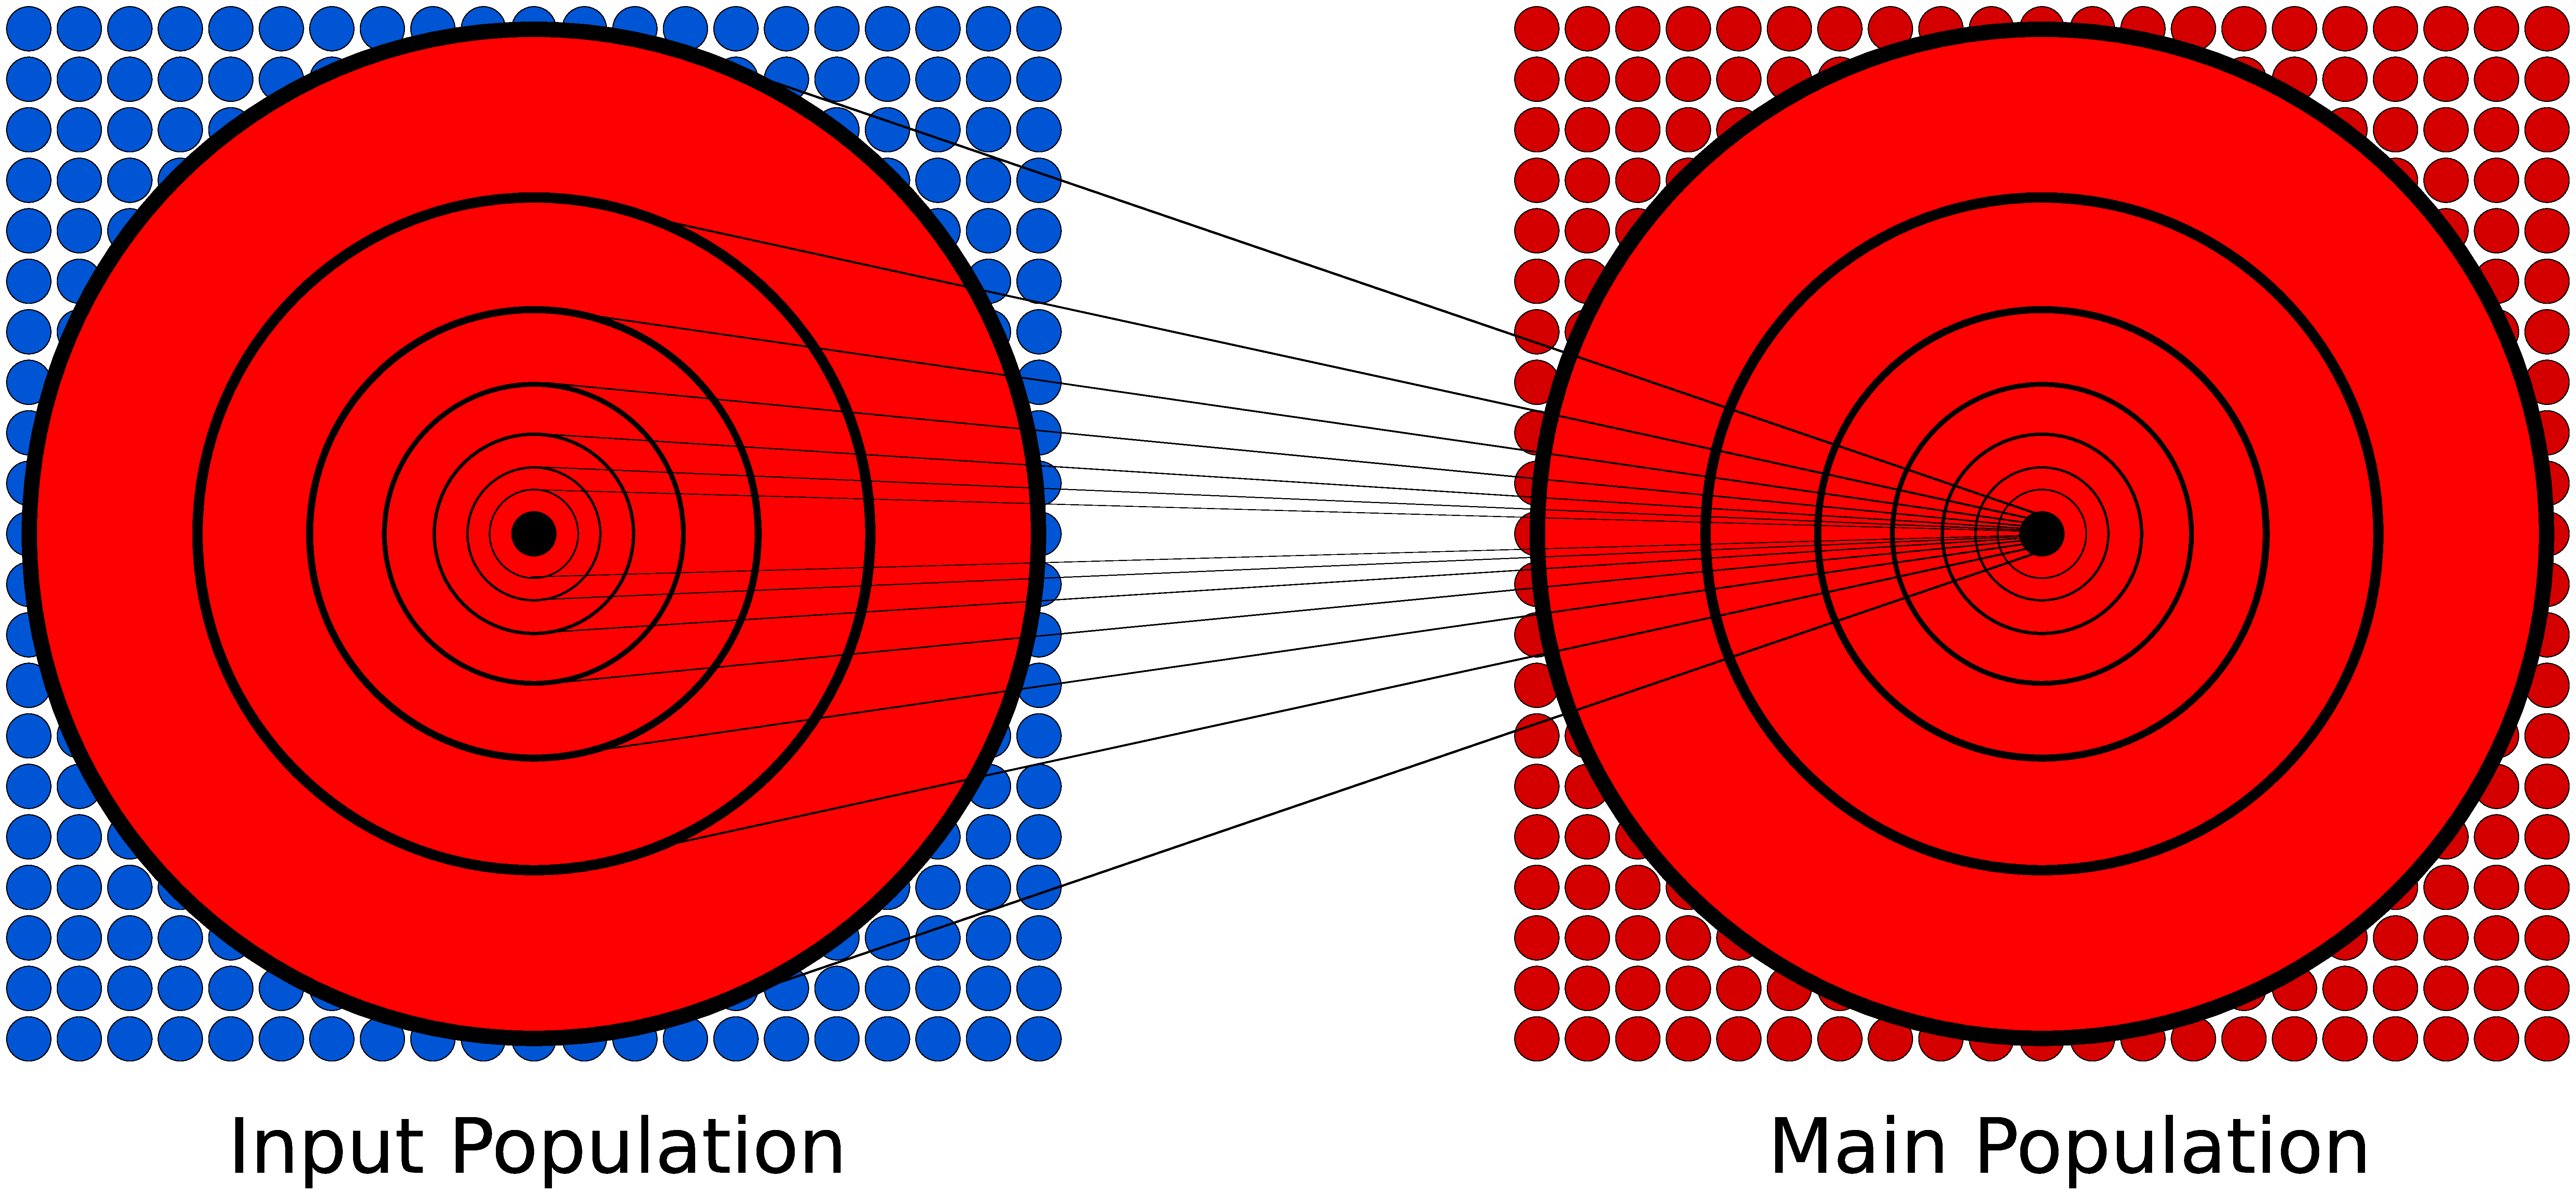
\includegraphics[width=7cm]{fieldsGaussians.eps}
  \caption{Neural fields for stability control}
\end{figure}



\section{Evolution of Neural Field Controllers for Biped Stability}
\subsection*{Evolutionary Algorithm Structure and Parameters}
For the evolution process it is used a simple evolutionary algorithm
as shown in the preliminaries, with random elimination of individuals
inversely proportional with its fitness.

% , but with the addition of niching in the for of Deterministic
% Crowding (see \cite{referencia-dc}), in order to promote additional
% diversity and to prevent premature convergence.

The evolution parameters are the connection kernels between the input
layer and the hidden layer, and between the hidden layer and the
output layer. The recurrent connections of the hidden layer with
itself are left fixed, in the form of a wizard hat function.

The connection kernels are considered isotropic and homogeneous along
the field, so that they can be described as symmetric one-dimensional
arrays of values.

\subsection*{Genotypic Representation and Evolution Operators}
Each connection kernel can be represented as an array of $N$ values
from $w(0)$ to $w(p)$ with homogeneous spacing, using its
symmetry. This way, for an equal boundary radius for all the kernels,
and a 3-layered architecture, there are $3N$ real values in the
genotype. As can be seen, the number of evolution parameters does not
have a direct relation with the simulation size of the neural fields
(the number of discrete points used), in contradistinction with
recurrent neural networks, where the number of parameters depends on
the number $n$ of neurons with a polynomial order $O(n^2)$.

\subsection*{Fitness Functions}
The fitness functions were selected in such a way that the stability
controller only has the goal to reduce inclination, while the
positioning controller has to take into account both inclination and
position. The fitness functions were tuned experimentally to attain a
convergence velocity suitable for the experiment. This has in mind a
notion of sequential evolution of, first, the capability to attain
equilibrium, and later, the capability to perturb the equilibrium
controller in such a way that a planned objective can be reached.

The fitness function for the stability controller is:

\begin{equation}
  F_1(\theta )=100-\frac{100\theta ^4}{\theta _{max}^4 T_{total}}
\end{equation}

And for the positioning controller is:

\begin{equation}
  F_1(\theta ,e_x)=100-\frac{100(\theta ^4+e_x^4)}{(\theta _{max}^4+e_{x,max}^4) T_{total}}
\end{equation}



\section{Experimental Set-up}
\label{sec:setup}

The model used consists of an approach to biped walking based on a
inverted pendulum (car-and-pole) system in which the pendulum
equilibrium is looked for. Nonetheless, supposing that the pendulum
mass represents the body center of mass, it is proposed that is
reasonable to expect a system with its sole function being to
stabilize the body. This way, the navigation system has as purpose to
carefully perturb the first controller in such a way that the
stabilizing controller moves the car to the desired position.

\subsection*{Dynamic Model}
The dynamic model used, in mathematical terms, is expressed in the two
equations:

\begin{align}
  \ddot{x}&=\frac{F+ml\dot{\theta}^2\sin\theta-mg\cos\theta\sin\theta}{M+m\sin^2\theta}\\
  \ddot{\theta}&=\frac{(M+m)g\sin\theta-F\cos\theta-ml\dot{\theta}^2\sin\theta\cos\theta}{l(M+m\sin^2\theta)}+\frac{\tau}{ml^2}
\end{align}

This model consists of four state variables and a high non-linearity
as it departs from equilibrium points. It is worth noting that the
wanted equilibrium point is in fact unstable.

\subsection*{RNN Controller Architecture for Comparison}
The proposed architecture for the recurrent neural network controller
has two expert recurrent networks, whose interaction will achieve
positioning and equilibrium as well.

There has been applied a preprocessing stage previous to the input
neurons, so that the actual values are not used and instead the inputs
are mapped to 3 fuzzy sets. In this way, the stability controller only
has 3 inputs, while the positioning controller has 6, corresponding to
the same 3 inputs previously described and another 3 due to the fuzzy
mapping of the error signal. All neurons are interconnected and the
first one of them is selected as output without loss of
generality. The neural network topology for the first controller
(stability) is shown in the figure \ref{fig:rnn-arch}.

\begin{figure}[t]
  \label{rnn-arch}
  \centering
  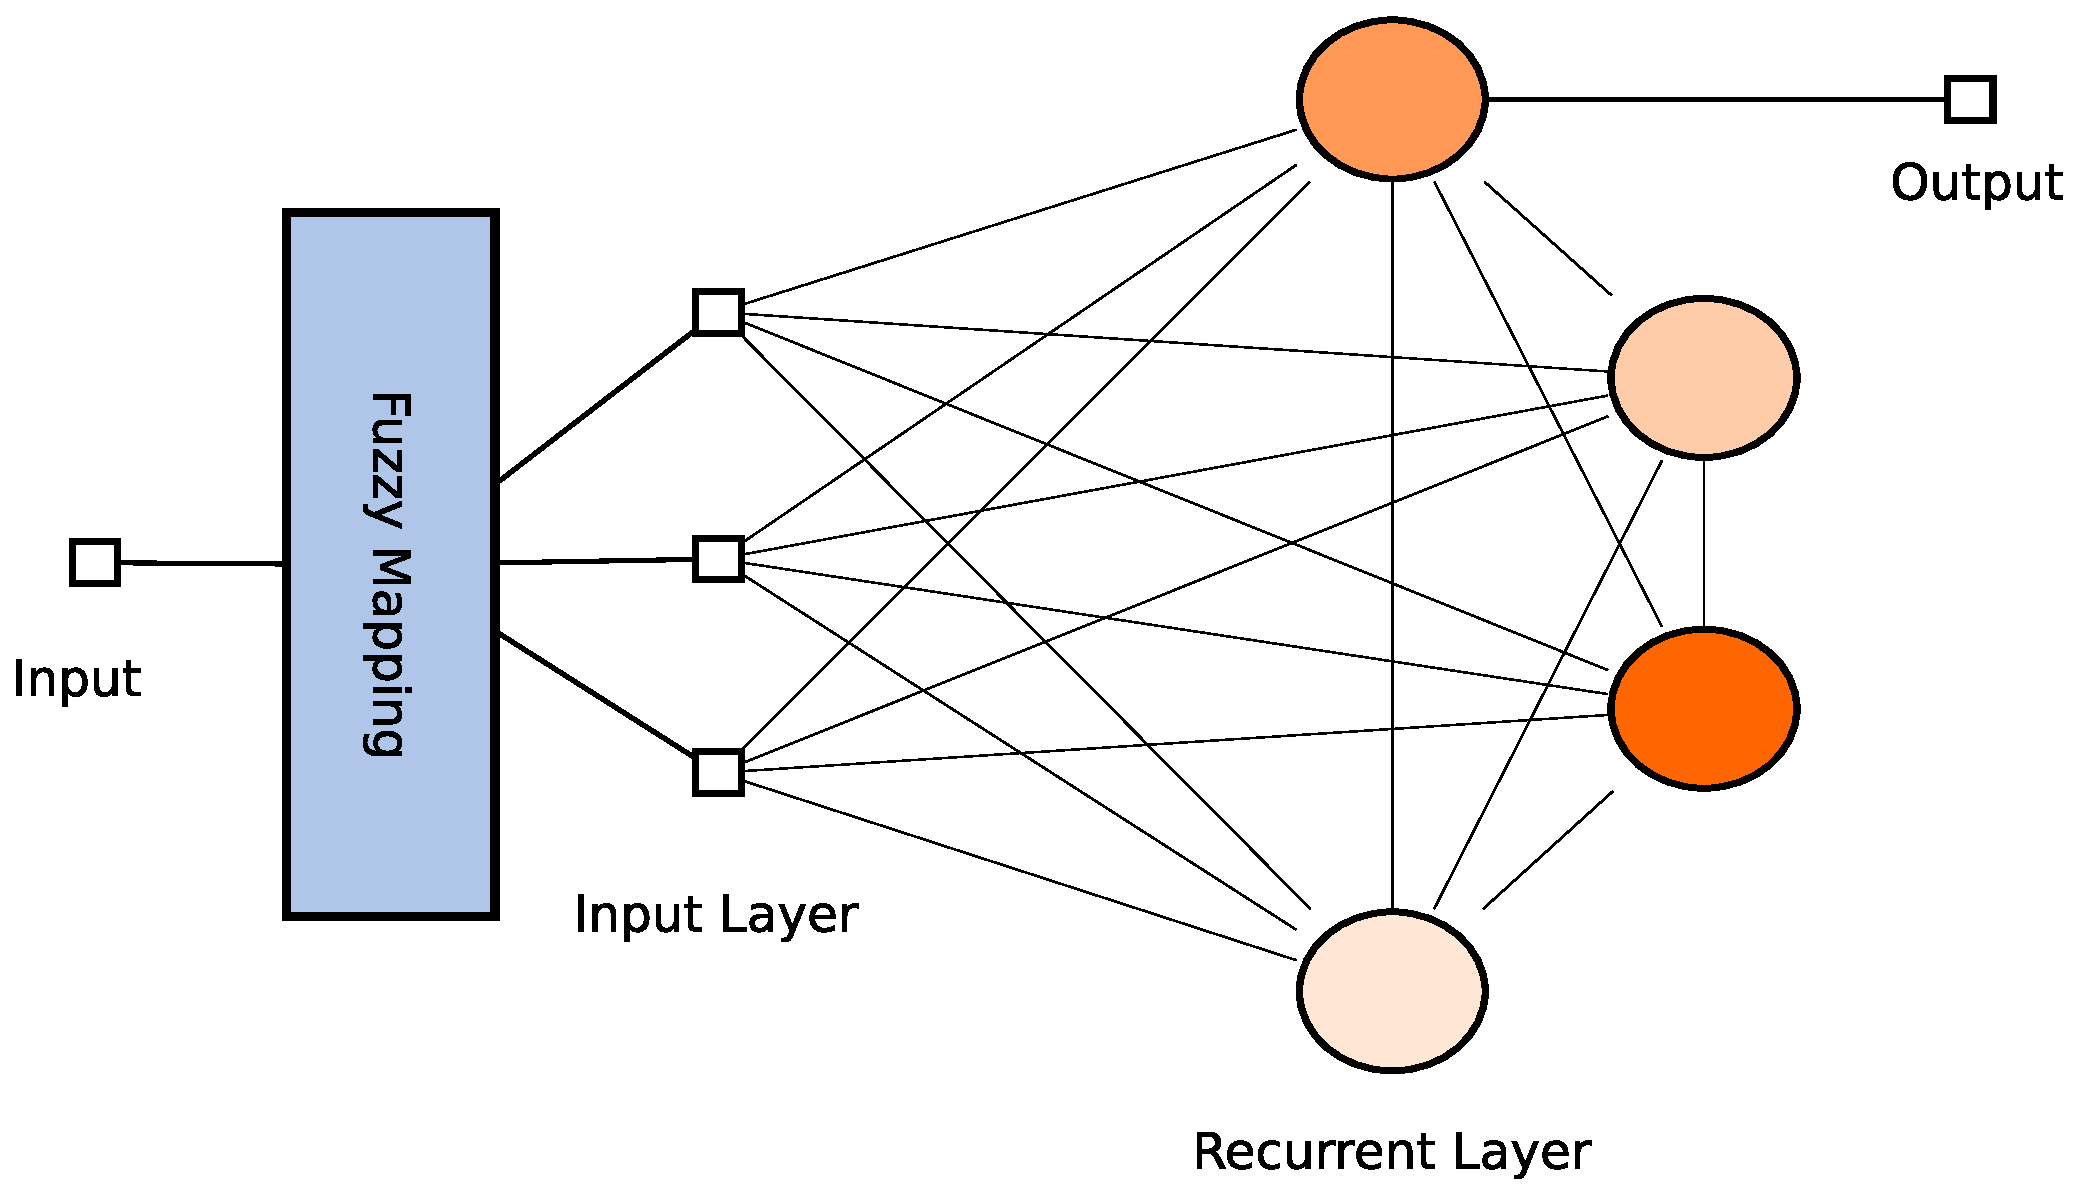
\includegraphics[width=7cm]{rnn.eps}
  \caption{Neural net for stability control including fuzzy mapping}
  \label{rnn}
\end{figure}

\subsection*{Evolutionary Algorithm Structure for the RNN Controller}
It is expected, based on the approach of artificial life to
evolutionary robotics (Nolfi y Floreano), that the sequential and
cooperative evolution of elements with biological similarity leads to
an specialization in the process of stabilization and positioning
(despite the antagonistic individual goals of each controller because
of the interest of the positioning controller to maximize also the
global performance).

As said, the two steps are executed sequentially, taking the best
individual of the first step to collaborate with the individual
evolved in the second step.

Aiming to obtain a fixed length representation and limit the problem
dimensionality, it is used a model of order $Q$ totally connected. Any
network with an order equal or lesser and with total or partial
connections can be represented by the proposed model, by the addition
of activating/deactivating elements for neurons and
connections. Therefore, individual are codified as:

\begin{itemize}
\item A bit sequence representing a serialization of an activation
  matrix $A_a$ of dimension $Q$-by-$Q$ which activates/deactivates a
  recurrent connection.
\item A sequence of real numbers representing a serialization of
  matrices $W_a$ and $W_b$, of dimension $Q$-by-$Q$ and $Q$-by-$(m+1)$
  respectively.
\end{itemize}

The $C$ matrix is not evolved because it is chosen arbitrarily only
one output (the first neuron).

The evolution operations used in both steps are:
\begin{itemize}
\item Parametric mutation of inputs: Gaussian modification of real
  codified matrix weights, which varies connection weights of inputs.
\item Parametric mutation of recurrences: Gaussian modification of
  real codified matrix weights, which varies connection weights of
  recurrences.
\item Selection: Calculates population fitness, selects with elitism
  and culling (5\% of both) couples of parents for generating new
  offsprings, calculates the fitness function for both offsprings.
\end{itemize}

The fitness functions used are the same presented for the neural field
controller.

\section{Experimental Results}
\subsection*{Experimentation Details}
The sampling time used was 0.04s (for neural networks, neural fields,
and visualization) and were performed 20s tests.

The differential equation system was solved by a numerical method, 4th
Order Runge-Kutta. The iteration step selected was $h=0.002s$ for each
test.

Here are shown the results for the proposed neural field architecture
without evolution and an appropriate selection of parameters (made
taking in account the self-stability of the neural fields and the time
constants of the plant), and the evolution of a recurrent neural
network of a recurrent neural network controller.

\subsection*{Results}
The first experiment tests the physical model using the recurrent
neural network controller without evolution, to see the natural
dynamics of the system when the controller is configured arbitrarily
(in such a way that can be perceived the need of the evolutionary
algorithm for the recurrent neural network controller). Results are
shown in the figure \ref{inestabilidad}. As can be seen, it is an
unstable system in the origin. Red dots represent the pendulum
position referenced to universal coordinates, and blue dots represent
the base (car) position.


\begin{figure}[t]
  \centering
  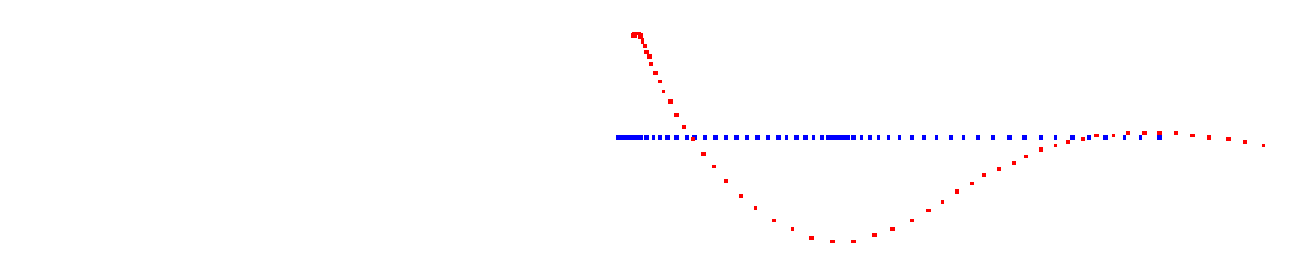
\includegraphics[width=7cm]{inestabilidadG.eps}
  \\
  \includegraphics[width=7cm]{inestabilidadC.eps}
  \caption{System dynamics with an untrained controller}
  \label{inestabilidad}
\end{figure}

After the first step of the algorithm, and once done the stability
controller evolution, it is shown the behavior withdrawing the
positioning controller in the figure \ref{final}. The evolution was
performed with a population of 50 individuals and 300 iterations.

\begin{figure}[t]
  \centering
  \includegraphics[width=7cm]{finalG.eps}
  \\
  \includegraphics[width=7cm]{finalC.eps}
  \caption{System dynamics with a RNN controller trained.}
  \label{final}
\end{figure}

On the other hand, when the initial angular perturbation is small, the
neural field is able to control the stability without evolution. The
simulation is shown in the figure \ref{estabilidad}.


\begin{figure}[t]
  \centering
  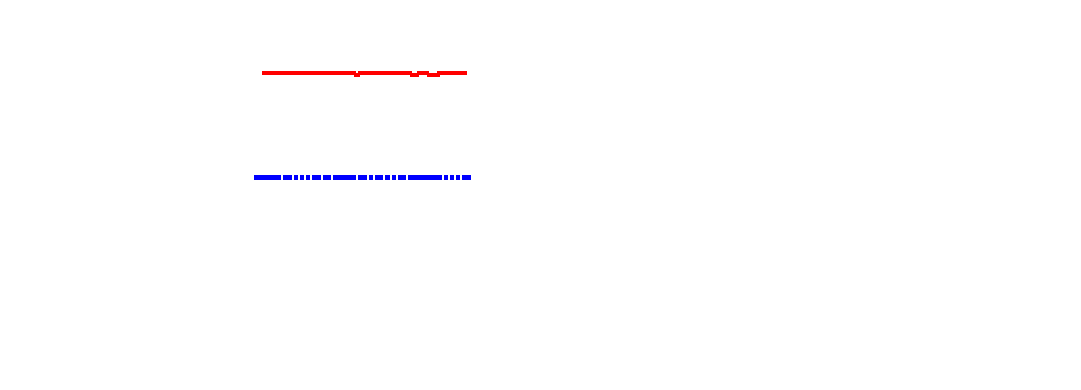
\includegraphics[width=7cm]{estabilidadG.eps}
  \\
  \includegraphics[width=7cm]{estabilidadC.eps}
  \caption{System dynamics with a non-trained Neural Field
    Controller.}
  \label{estabilidad}
\end{figure}

The output from the processing field can be seen in the figure
\ref{fig:nf-result}.


\begin{figure}[t]
  \centering
  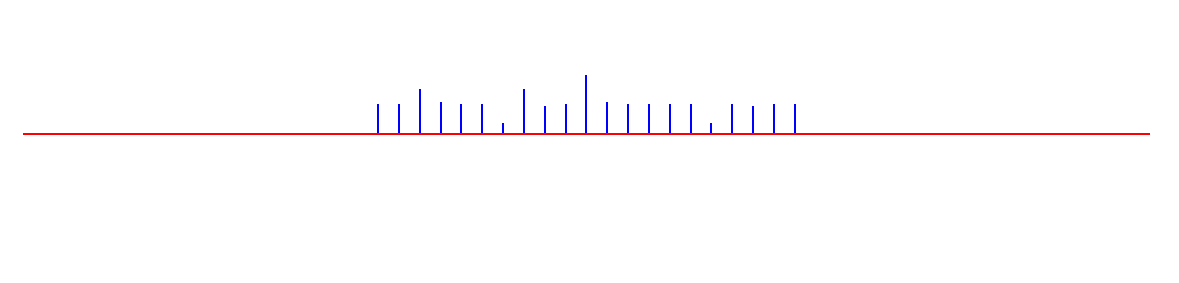
\includegraphics[width=7cm]{camposC.eps}
  \caption{Processing Neural Field simulation.}
  \label{estabilidad}
\end{figure}



\section{Conclusions}
The results obtained from this chapter can be summarized in a short
analysis.

While the recurrent neural network controller is expressive enough to
solve the problem at hand, the number of parameter to configure (or in
this case to evolve) is of a quadratic order in relation to the number
of nodes (or neurons). This were not a particular problem for the
evolutionary algorithm used, but limits its potential
scalability. Furthermore, while it is expressive enough, does not show
a particular suitability to the dynamic stability problem of the
inverted pendulum and there are no reasons to expect something
different for a more complex biped model.

On the other hand, the neural field controller is a bit more complex
and its simulation more costly, but has some notable advantages. The
first one is its ability to self-compensate or, equivalently, the
stability of its natural dynamics, which is attained after the setup
of few parameters. The second one is it suitability to the problem at
hand, being able to solve it with a acceptable degree of performance
for small perturbations. Although there was a need to parameter
configuration, evolution was not required because the small number of
parameters to setup: basically three parameters of the kernel function
and the resting potential of the field equation - a number of
parameters of constant order in relation to the number of nodes (point
potentials on the neural field).

It is left for future work the challenging but promising task of
neural field evolution.

\bibliographystyle{IEEEtran.bst}
% \bibliographystyle{natbib}
\bibliography{bibanot}

% \begin{thebibliography}{}
% \bibitem[RN] {RN} Stuart Russell and Peter Norvig (2003)
%   \textit{Artificial Intelligence: A Modern
%     Approach}. Prentice-Hall, Englewood Cliffs, NJ.
% \bibitem[Ha] {Ha} Simon Haykin (1994) \textit{Neural networks: a
%     comprehensive foundation} Macmillan.
% \bibitem[NF] {NF} Stefano Nolfi and Dario Floreano (2004)
%   \textit{Evolutionary Robotics: The Biology, Intelligence, and
%     Technology of Self-Organizing Machines} Bradford Book.
% \end{thebibliography}

\end{document}
